\documentclass{article}

\usepackage[final]{nips_2017}
\usepackage[utf8]{inputenc} % allow utf-8 input
\usepackage[T1]{fontenc}    % use 8-bit T1 fonts
\usepackage{hyperref}       % hyperlinks
\usepackage{url}            % simple URL typesetting
\usepackage{booktabs}       % professional-quality tables
\usepackage{amsfonts}       % blackboard math symbols
\usepackage{nicefrac}       % compact symbols for 1/2, etc.
\usepackage{microtype}      % microtypography
\usepackage{pdfpages}       % Because LaTeX doesn't take SVGs...
\usepackage{amsmath}
\usepackage{algorithm}
\usepackage{algorithmic}
\usepackage{natbib}


\title{Pulsar Classification using Deep Neural Networks}

\author{
    Kyle W.~MacMillan
    Department of Computer Science\\
    South Dakota School of Mines and Technology\\
    Rapid City, SD 57701 \\
    \texttt{kyle.macmillan@mines.sdsmt.edu} \\
}

\begin{document}

\maketitle

\begin{abstract}
    Pulsars are rapidly rotating, highly magnetized, neutron stars and white 
    dwarfs that emit focused electromagnetic radiation in a beam. The beam is 
    only visible to us when it is directly facing Earth and is the reason for 
    their pulsed nature. This paper approaches classification of pulsars and 
    non-pulsars with the intent of learning more about TensorFlow. The 
    classification method used is Deep Neural Networks and an acceptable level 
    of accuracy was obtained.
\end{abstract}

\section{Introduction}
    We were tasked with picking a dataset and training a deep learning network. 
    First thing to do was to pick a dataset. Being an open-ended assignment 
    there was uncertainty as to what particular dataset to explore. Initial 
    looks involved different image classification datasets such as CIFAR-10, 
    Caltech 101, and NORB. Down the road there is no desire to work with image 
    data classification, work with files and datasets of continuous and 
    discrete data are preferred. After thorough search of the available 
    datasets it was decided pulsar classification provided by 
    \citet{orig_pulsar} was best suited this paper. 

    The last decision before pressing on to data format was to pick the correct 
    deep learning framework for the job. There were several options but 
    TensorFlow seemed like a good choice. Keras and PyTorch are other tools 
    that utilize TensorFlow but were not used because those are often 
    considered a "front end" for TensorFlow, which was not part of the goals of 
    the assignment.

\section{Method}

\subsection{Main}
    Main.py is where the project is ran from. There are several hyperparameters 
    that a user can pick, beginning with $\_TEST\_PERCENTAGE$, which sets the 
    percentage of comma-separated values (CSV) data to be utilized for testing. 
    Industry standard is 20\%, so that is the default setting. The training 
    data $\_TRAIN$ is, as a result, 80\% of the CSV data. 
    % 
    \[\mathcal{\_TRAIN}=\_NUM\_ELEMENTS * ( 1 - \_TEST\_PERCENTAGE )\]
    % 
    It was necessary to hard-code in the number of elements in the CSV file 
    because there was trouble when trying to run update on the CSV class due to 
    an incomplete understanding of python abilities such as $class.update()$.

    $\_BATCH\_SIZE$ is set as 
    %
    \[\mathcal{\_BATCH\_SIZE}=max\{\_TRAIN*0.1, 1\}\]
    %
    This is part of ensuring the training does not get stuck in local minima. 
    \_MODEL is then set as whichever optimizer the user would like, in this 
    case, RMSPropOptimizer was selected. A CSV class is created based on the 
    dataset to be classified. 

    Hyperparameter choices are part of the art of machine learning but in this 
    project it was not the focus to make perfect hyperparameters. That being 
    said, that was explored briefly for this project as seen in section 
    \ref{sec:hyperparams}. $\_NODES\_PER\_LAYER$ was one of such 
    hyperparameters, as was $\_LAYERS$, and $\_HIDDEN\_LAYERS$. The final 
    implementation of these parameters are as follows:
    %
    \[\mathcal{\_NODES\_PER\_LAYER}=(num\_features - 1) * 1.5\]
    \[\mathcal{\_LAYERS}=max\{sqrt(\_NODES\_PER\_LAYER), 2\}\]
    \[\mathcal{\_HIDDEN\_LAYERS}=[\_NODES\_PER\_LAYER] * \_LAYERS\]
    %
    This lead to 3 hidden layers with 12 nodes each for the \href{https://archive.ics.uci.edu/ml/datasets/HTRU2}{HTRU\_2 Dataset}.

    After all parameters have been setup main gets run. Users can select the 
    number of runs to perform as an argument when they begin the program e.g. 
    %
    \[\textnormal{python\ main.py \textit{X}}\]  
    %
    The program will then run the classifier \textit{X} times. After finishing 
    the program will output classification accuracy of the given dataset.



\subsection{Data format}
    After determining the dataset and the framework to be utilized it is 
    necessary to figure out how to read data from the dataset. A modular 
    approach was taken with this project. Users will be able to select a CSV 
    file to load in. By specifying a class to contain the CSV data it is 
    possible to run multiple datasets while making only minor modifications to 
    the code. The format is also much easier to read as a result of the class 
    format.

    Rather than code up a custom method of moving CSV data into a format usable 
    by the deep learning framework it was determined to "stand on the shoulders 
    of giants". Pandas was used to bring CSV data into usable form. After 
    pulling the data into a single structure it was necessary to split the data 
    into training and testing data. Again, rather than code that from scratch 
    it was determined best practice to utilize existing tools. 

    For that endevour scikit-learn was used, specifically the 
    $train\_test\_split()$ method. As is standard for classification problems 
    the data was segmented into 80\% training and 20\% testing data. It was 
    then necessary to place the $class$ label into a data structure for later. 
    For both the train and test data, associated labels are passed, along with 
    the data, as tuples. The psuedocode for this section can be found under 
    Algorithm \ref{alg:input_fn}.
    %
    \begin{algorithm}
        \caption{$input\_fn()$}
        \label{alg:input_fn}
        \begin{algorithmic}
            \STATE $data \gets CSV$\\
            \STATE $test, train \gets train\_test\_split(data)$
            \STATE $test\_label \gets test.pop(class)$
            \STATE $train\_label \gets train.pop(class)$
            \RETURN $(train, train\_label), (test,test\_label)$
        \end{algorithmic}
    \end{algorithm}
    %

\subsection{TensorFlow estimator}
    TensorFlow has built in estimators such as:
    %
    \begin{itemize}
        \item \href{https://www.tensorflow.org/api_docs/python/tf/estimator/DNNClassifier}{DNNClassifier}
        \item \href{https://www.tensorflow.org/api_docs/python/tf/estimator/BaselineClassifier}{BaselineClassifier}
        \item \href{https://www.tensorflow.org/api_docs/python/tf/estimator/BaselineRegressor}{BaselineRegressor}
        \item \href{https://www.tensorflow.org/api_docs/python/tf/estimator/DNNLinearCombinedClassifier}{DNNLinearCombinedClassifier}
        \item \href{https://www.tensorflow.org/api_docs/python/tf/estimator/LinearClassifier}{LinearClassifier}
        \item \href{https://www.tensorflow.org/api_docs/python/tf/estimator/LinearRegressor}{LinearRegressor}
    \end{itemize}
    %
    You also have the ability to build your own estimator, or classifier, and 
    this is the route that was selected for this project. The custom estimator 
    selected utilizes the $model$ specified at the start of the program, a 
    $model\_dir$ for TensorBoard output which will be discussed in section 
    \ref{sec:tensorboard}, and the $params$ which consist of 
    $feature\_columns$, $hidden\_units$, and $n\_classes$.

    Estimator also requires \href{https://www.tensorflow.org/versions/r1.2/api_docs/python/tf/estimator/ModeKeys}{three modes} depending on the goal:
    %
    \begin{itemize}
    \item ModeKeys.TRAIN
    \item ModeKeys.EVAL
    \item ModeKeys.PREDICT
    \end{itemize}
    %
    Lastly, the estimator requires a return of $EstimatorSpec$. Documentation 
    for the EstimatorSpec can be found on \href{https://www.tensorflow.org/api_docs/python/tf/estimator/EstimatorSpec}{TensorFlow's website}. It is important to note 
    that each of the different $ModeKeys$ requires a different set of 
    parameters for the returned $EstimatorSpec$.

\subsection{Training}
    TensorFlow offers the ability to train estimators by calling a $train()$ 
    method. For this paper the $input\_fn$ and $steps$ arguments are set by a 
    function call to $train\_input\_fn$ and $csv.num\_examples['train']$ 
    respectively. This allows the data to be segmented for training.

    The model that was instantiated during estimator creation is detailed under
    $\textnormal{model.model\_RMSProp}$. For each of the layers that was passed 
    to it under $params['hidden\_units']$ there is a fully connected layer 
    built with selu activation. \citet{selu} found with the proper math you can 
    obtain self-normalizing exponential linear units, meaning they don't 
    require batch normalization and that is why they were chosen over all of 
    the other activation functions. There is also the final fully connected 
    layer which has no activation layer. This final layer aids in determining 
    the classification.

    During training ModeKeys.TRAIN is called, which specifies RMSProp gradient 
    descent as our optimizer and then calls $minimize()$. The $minimize()$ 
    method will automatically compute the gradients and apply them to the 
    variables, but if you need to tune the network there are additional steps 
    that can be taken instead:
    %
    \begin{enumerate}
        \item Compute the gradients with $compute\_gradients()$
        \item Process the gradients as you wish
        \item Apply the processed gradients with $apply\_gradients()$
    \end{enumerate}
    %
    Further documentation on this process can be found on TensorFlow's website 
    under the \href{https://www.tensorflow.org/api_docs/python/tf/train/Optimizer}
    {class Optimizer}. It was not necessary to have that level of fidelity with 
    this particular dataset, so the base $minimize()$ was all that was 
    necessary.

    With $minimize()$ minimizing the loss we are able to make progress towards 
    a classification. This dataset in particular minimizes loss to near-zero 
    after just the first episode of 100 training steps as can be seen in Figure 
    \ref{img:loss}.


\subsection{Hyperparameters}\label{sec:hyperparams}
    Hyperparameters are normally very important but in this dataset it was 
    discovered that they had very little impact on the efficacy of 
    this classifier.

    An example of hyperparameter randomization can be found under:
    %
    \[\textnormal{python\ hyperparams.py}\]
    %
    That file will automatically generate randomized hyperparameters. During 
    testing of this project various hyperparameters were tested with no 
    significant improvements over the initial parameters set so the associated 
    code was removed from primary operation of the classifier. The file 
    described would allow for random testing of hyperparameters across any 
    number of computers. \citet{hypparam} found random search of 
    hyperparameters to be superior to grid search and was the method used while 
    exploring hyperparameter tuning during this project.

\subsection{TensorBoard}\label{sec:tensorboard}
    One of the other reasons for utilizing TensorFlow is the TensorBoard 
    project. TensorBoard allows for visualization of various parameters as 
    defined by the user. Figure \ref{img:acc_smooth} and \ref{img:loss_smooth} 
    are the same results as shown in Figure \ref{img:accuracy} and 
    \ref{img:loss} respectively. The smooothing helps in understanding what may 
    be going on, especially in more turbulant graphs. Another benefit is being 
    able to visualize the graph structure. To use TensorBoard on this project 
    ensure it was installed with TensorFlow and type 
    %
    \[\textnormal{tensorboard\ -\--logdir\ model}\]
    %
    and go to the link it provides (by ctrl clicking or copy/paste). 
    %
    \begin{figure}[H]  
    \begin{center}
    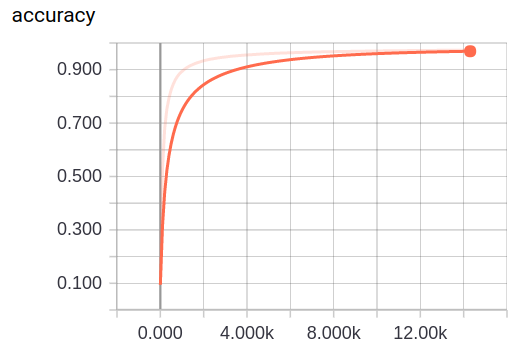
\includegraphics[scale=0.65]{images/acc}
    \caption{Smoothed accuracy}\label{img:acc_smooth}
    \end{center}
    \end{figure}
    %
    \begin{figure}[H]  
    \begin{center}
    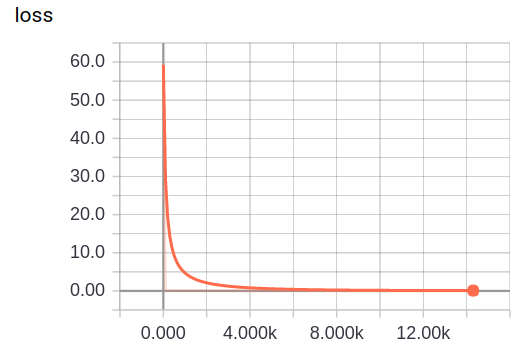
\includegraphics[scale=0.65]{images/loss}
    \caption{Smoothed loss}\label{img:loss_smooth}
    \end{center}
    \end{figure}
    %
\newpage
\section{Results}\label{sec:results}
    RMSProp gradient descent with 0.001 learning rate, performing batch runs on 
    10\% of the training samples every 100 steps produced an accuracy of 97.8\% 
    averaged over 20 tests. These were taken with 80\% train and 20\% test 
    samples. Other hyperparameters were three fully connected layers with 12 
    nodes each using selu activation. Increasing hidden layers led to noisier 
    loss after the large initial drop. The following had no measurable 
    improvement on the classification accuracy:
    \begin{itemize}
        \item Changing from RMSProp to Adagrad
        \item Changing batch size
        \item Modified learning rate
        \item Depth of layers or number of neurons
    \end{itemize}
    %
    \begin{figure}[H]  
    \begin{center}
    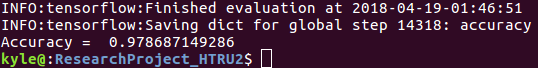
\includegraphics[scale=0.735]{images/accuracy_percent_small}
    \caption{Detailed accuracy}\label{img:term_acc}
    \end{center}
    \end{figure}
    %
    \begin{figure}[H]  
    \begin{center}
    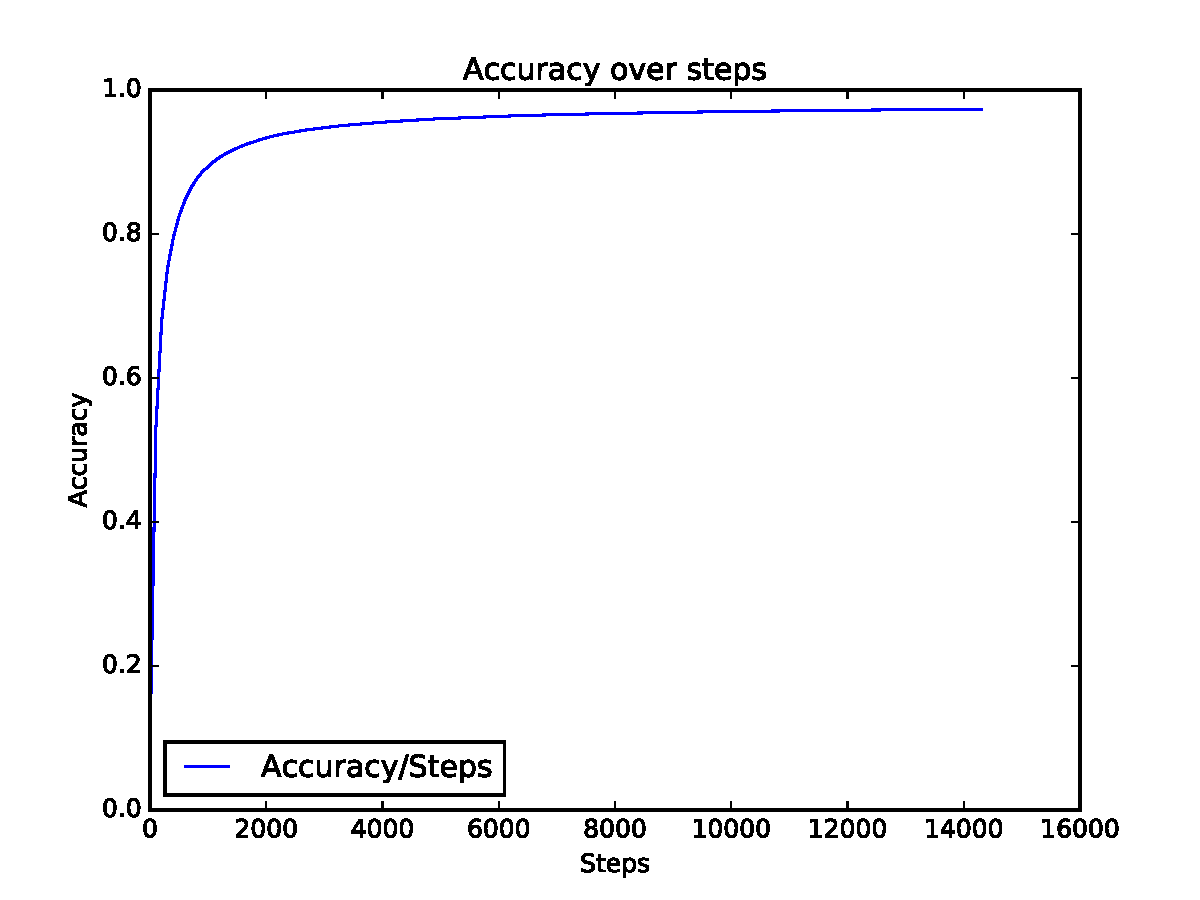
\includegraphics[scale=0.75]{images/Accuracy}
    \caption{Accuracy}\label{img:accuracy}
    \end{center}
    \end{figure}
    %
    \begin{figure}[H]
    \begin{center}
    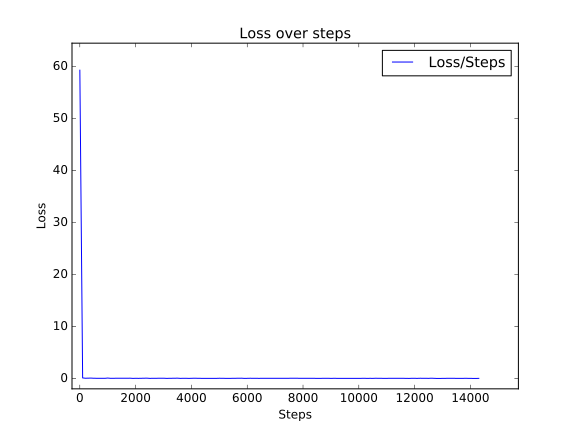
\includegraphics[scale=0.75]{images/Loss}
    \caption{Loss}\label{img:loss}
    \end{center}
    \end{figure}
    %
\section{Conclusion and future work}
    In conclusion, this particular dataset ended up being relatively simple to 
    classify with modern methods. The original paper reported the exact same 
    accuracy of 97.8\% using a Gaussian Hellinger Very Fast Decision Tree. Room 
    for improvement could be a better interface for the CSV files and possible 
    command line arguments. Additionally, the accuracy would occasionally break 
    98\%, but was rare. There is possible room for improvement on the 
    hyperparameters to increase the accuracy consistently beyond 98\%. The loss 
    function dropped off almost immediately, so it could probably deal with 
    fewer hidden layers and/or neurons. Another possible improvement may be 
    adding extra feature layers that are extrapolated from the pulsars (or 
    possibly non-pulsars).
    
\bibliographystyle{plainnat}
\bibliography{bib}
\end{document}